\documentclass[a4 paper]{article}
% Set target color model to RGB
\usepackage[inner=2.0cm,outer=2.0cm,top=2.5cm,bottom=2.5cm]{geometry}
\usepackage{setspace}
\usepackage[rgb]{xcolor}
\usepackage{verbatim}
\usepackage{subcaption}
\usepackage{amsgen,amsmath,amstext,amsbsy,amsopn,tikz,amssymb,tkz-linknodes}
\usepackage{fancyhdr}
\usepackage[colorlinks=true, urlcolor=blue,  linkcolor=blue, citecolor=blue]{hyperref}
\usepackage[colorinlistoftodos]{todonotes}
\usepackage{rotating}
\usepackage{float}

\usepackage{booktabs}
\newcommand{\ra}[1]{\renewcommand{\arraystretch}{#1}}

\newcommand{\homework}[6]{
   \pagestyle{myheadings}
   \thispagestyle{plain}
   \newpage
  

  \pagestyle{fancy}
  \fancyhead[RO,LE]{\thepage}
  \fancyhf{} % clear all fields

  
   \setcounter{page}{1}
   \noindent
   \begin{center}
   \framebox{
      \vbox{\vspace{2mm}
    \hbox to 6.28in { {\bf COL331:~Operating Systems \hfill { #2}} }
       \vspace{6mm}
       \hbox to 6.28in { {\LARGE \hfill #1  \hfill} }
       \vspace{6mm}
       \hbox to 6.28in {\bf {Entry Number: {\rm #4} \hfill Name: {\rm #5} } }
       % \hbox to 6.28in { {\it TA: #4  \hfill #6}}
      \vspace{2mm}}
   }
   \end{center}
   \lhead{#1}
   \rhead{Page \thepage}
   % \markboth{#1}{#1}
   \cfoot{\thepage}
   \vspace*{4mm}
}

% \newcommand{\problem}[2]{~\\\fbox{\textbf{Problem #1}}\hfill (#2 points)\newline\newline}
% \newcommand{\subproblem}[1]{~\newline\textbf{(#1)}}
% \newcommand{\D}{\mathcal{D}}
% \newcommand{\Hy}{\mathcal{H}}
% \newcommand{\VS}{\textrm{VS}}
% \newcommand{\solution}{~\newline\textbf{\textit{(Solution)}} }

% \newcommand{\bbF}{\mathbb{F}}
% \newcommand{\bbX}{\mathbb{X}}
% \newcommand{\bI}{\mathbf{I}}
% \newcommand{\bX}{\mathbf{X}}
% \newcommand{\bY}{\mathbf{Y}}
% \newcommand{\bepsilon}{\boldsymbol{\epsilon}}
% \newcommand{\balpha}{\boldsymbol{\alpha}}
% \newcommand{\bbeta}{\boldsymbol{\beta}}
% \newcommand{\0}{\mathbf{0}}

\begin{document}
\homework{Assignment 2 Report}{Date: March 22, 2019}{}{\bf 2016CS10363}{\bf Manish Tanwar}{NetId(s)}

\section*{Part 1 - Jacob:}
\subsection*{Plot - Time Vs the number of processes:}

\begin{figure}[H]
	\centering %width=90mm
	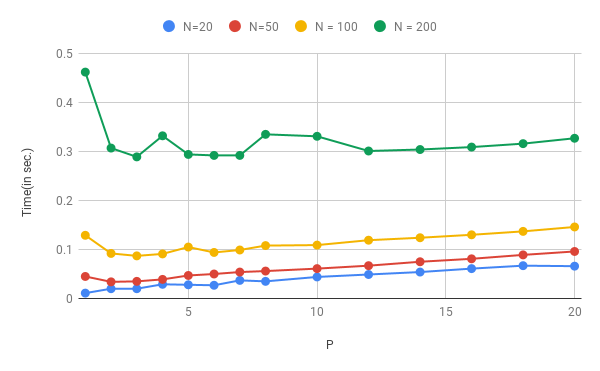
\includegraphics[width=160mm]{Jacob_time_P.png}
	\caption{Time Vs the number of processes\label{MIMD}}
\end{figure}

\subsection*{Plot - Speedup Vs the number of processes:}

\begin{figure}[H]
	\centering %width=90mm
	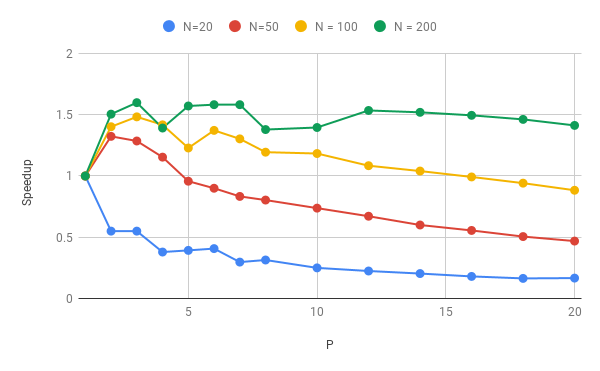
\includegraphics[width=160mm]{Jacob_speedup_P.png}
	\caption{Speedup Vs the number of processes\label{MIMD}}
\end{figure}

\subsubsection*{Observations:}
\begin{itemize}
\item As we increase the number of process first computation increases and then decreases. Decrease is the result of overhead of IPC communication.
\item The algorithm is scalable as the speedup increases in a better trend for large value of $N$.
\end{itemize}

\section*{Part 2 - Maekawa:}
\subsection*{Plot - Time Vs the number of processes:}
\begin{figure}[H]
	\centering %width=90mm
	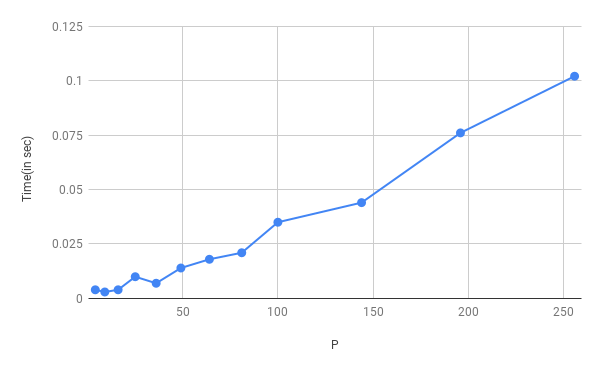
\includegraphics[width=160mm]{mak.png}
	\caption{Time Vs the number of processes(P = P3, P1 = P2 = 0)\label{MIMD}}
\end{figure}

\subsubsection*{Observations:}
\begin{itemize}
\item As we increase the number of processes the time increases.
\item Maekawa algorithm requires $O(\sqrt{n})$ messages for implementing mutual exclusion.
\item $O(\sqrt{n})$ trend can be observerd in the plot for small values of $P$, but as $P$ further increases due to more overhead time is more than $O(\sqrt{n})$.
\end{itemize}

\subsubsection*{Correctness:}
\begin{itemize}
\item For Jacob algorithm, ran the parallel version against the provided serial code for several testcases. 
\end{itemize}

\end{document} 